\chapter{Models for  Search-Encounter Data}
\markboth{Search-Encounter}{}
\label{chapt.searchencounter}

\vspace{0.3cm}


In this chapter we discuss models for 
search-encounter data. These are models that arise where you get
actual location data of individuals not biased by trap locations but
rather by searching space in some fashion. In most cases both
detection probability and movement parameters are resolvable. i.e.,
models that preserve the these movement outcomes -- the $u_{it}$ variables.
The models we differentiate here depend on a number of
things related to data structure or protocol -- basically whether or
not we record the exact location and how we record it. All models have
an underlying movement model which may be completely latent or not.

How exactly
are these different from models for data from fixed arrays?  (1)
sample units are either continuous space polygons or lines, not
points; (2) we have location information that is not biased by trap
locations (but is biased by the observation device somehow); (3)
because we have direct observations of location that exist independent
of traps we can often build an explicit model of space usage or an
explicit movement model.

A few variations of the models exist -- a long sample path through a
sample region where we note the locations of individuals seen along
the way, {\it and their identity} (this is different from distance
sampling int hat sense). Or we could search a region systematically
and so forth.  
The canonical situation is Royle and Young (2008) which involved a
plot search for lizards. They assumed the plot was uniformly searched
which justified the assumption of constant $p$ within the plot
boundaries. The data set was $\ge 1$ location observations for each of
a sample of $n$ individuals. 
The recent paper by Efford XXXX
discussed likelihood analysis of similar models. In the jargon of
\mbox{\tt secr} such models are referred to as models for {\it polygon detectors}.
 An extension of this model was described
by \citep{royle_etal:2011mee}.  

Search-encounter models also provide something of a bridge between the
standard models for fixed trap arrays (e.g., Chapt. \ref{chapt.scr0}),
and the models of \citep{chandler_royle:2012} where no individual
identity is present. The latter are search-encounter models where the
movement process (and outcomes) are completely latent. Another type of
model is SCR/DS -- this is a SCR model with ..................

\section{Search-Encounter sampling designs}

For our purposes here we recognize 4 basic sampling designs, each of
which might have variations due to modification of the basic sampling
protocol. In later sections of this chapter we will do some examples
but not of all of them.

{\flushleft \bf Design 1: Fixed Search Path.}  The ideal situation is
where we have a continuous search-path or lines, or multiple such
lines, in some region (Fig. XXXX 1 XXXXX). This is the type of problem described
by Royle et al. (2011 MEE). We assume the path or lines are laid out a
priori in some manner that is done independent of the activity centers
of individuals and the collection of data does not affect the
lines. Sometimes the lines are within well-defined polygons but the
polygon boundaries are not meaningful in terms of the observation
process.  A number of variations of the data collection protocol are
possible:
\begin{itemize}
 \item[] Protocol (1a) has us just record the locations of individuals
 \item[] Protocol (1b) has us record location of individuals AND
   location on the transect where we observed the individual
 \item[] Protocol (1c) has us record neither of those things, instead
   we record the closest perpendicular distance. This is a typical
   distance sampling situation which produces exactly a DS type of a
   model (or a CR-DS model). We don't recommend recording closest
   perpendicular distance and we don't discuss these models too much
   here
 \item[] Protocol (1d) . In this case, observations are restricted to
   the line itself. We imagine that the line is evolving in response
   to search activity. It is not quite like the other ones so let's
   call it ``ad hoc''. In this case we use small bins as traps and the
   length of the line in each grid as a covariate. Unstructured survey
   data. Thompson et al. and Russell et al.
 \end{itemize}


\begin{figure}
\centering
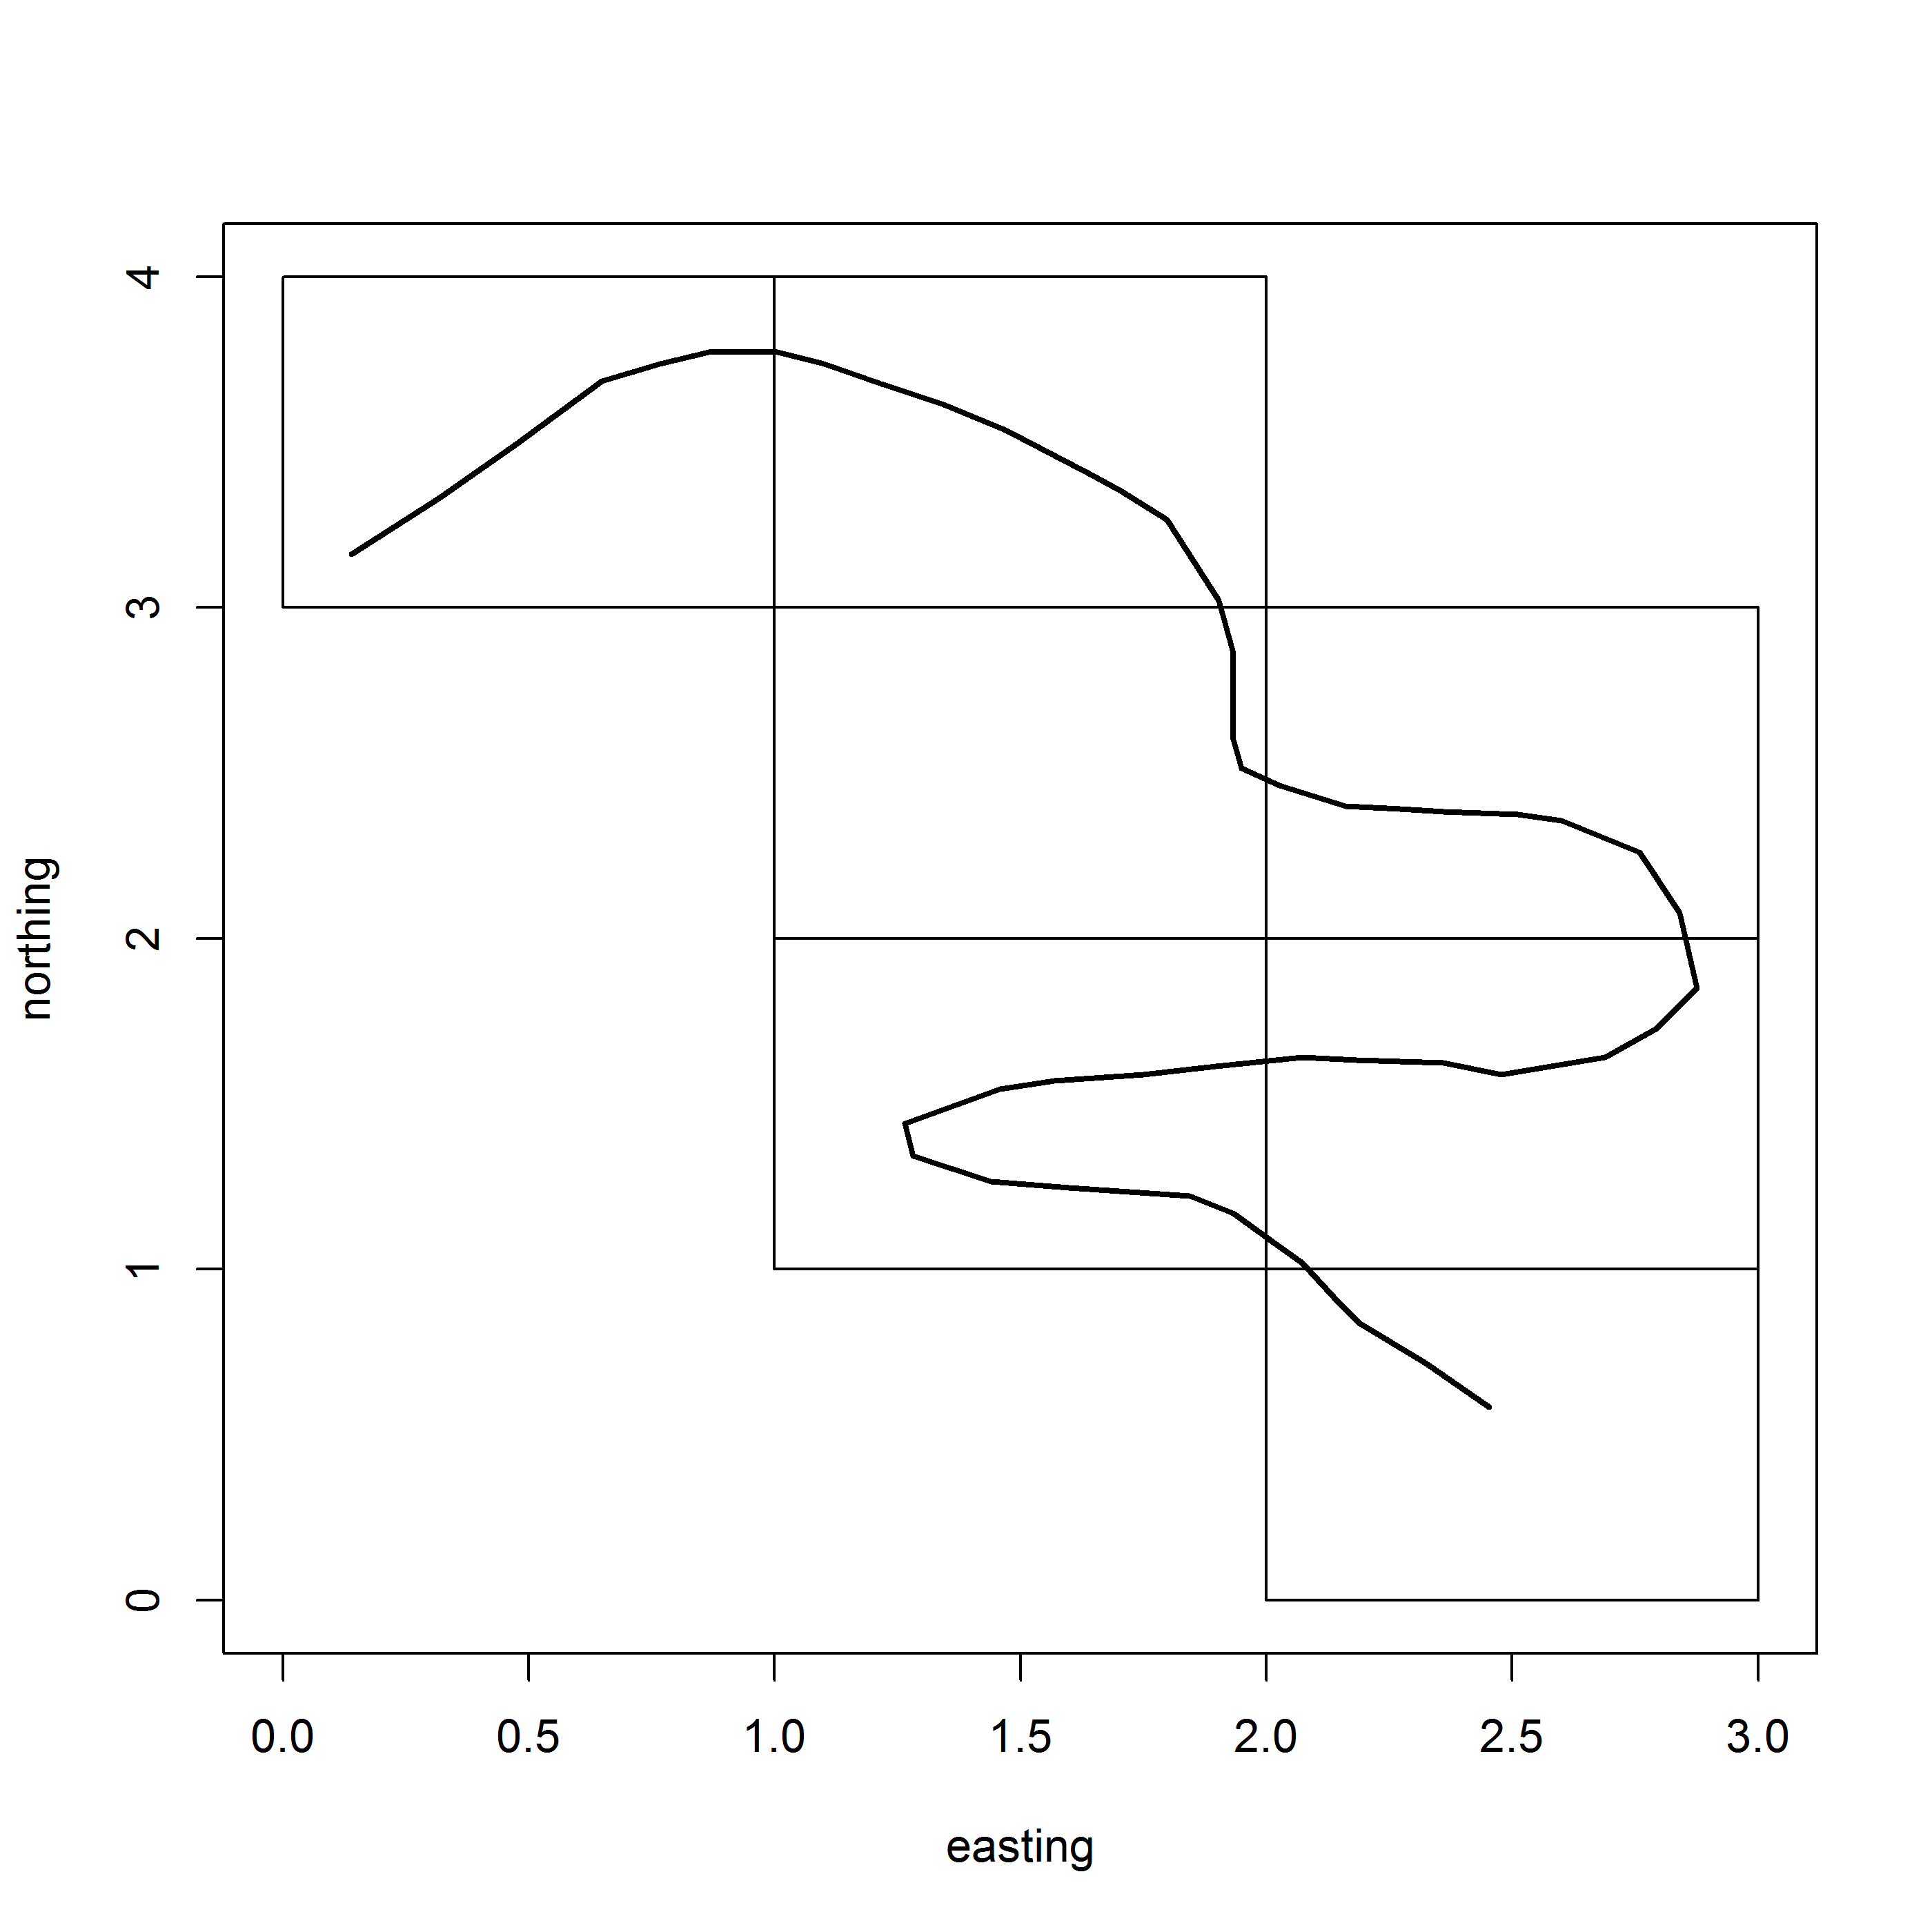
\includegraphics[width=4in,height=4in]{Ch16-searchencounter/figs/snakeline.png}
\caption{snake line.... showing design 1. more here.
}
\label{searchencounter.fig.snakeline}
\end{figure}



{\flushleft \bf Design 2: Uniform search intensity.}  In this case we
have one or more well-defined sample areas (polygons), such as a
quadrat or a transect, and we imagine that the area is uniformly
searched so that $p = p_0$ is constant within the search area.
Sampling produces locations of individuals within the well-defined
boundaries of the sample area. The polygon boundaries defining the
sample unit are important because it tells us that $p=0$ by design
outside of the boundary.

Using the example from the Figure above, we could imagine that each
quadrat was uniformly searched. The individual quadrat boundaries are
irrelevant and we only need to be concerned about the ``total''
boundary of the composite polygon (the intersection of all little
ones). That said for analysis in BUGS it is easier to work with square
polygons.  We show a simulation example here and we analyze it either
using a bivariate normal movement model or else a 2-d random walk type
of model.  But we don't provide a real example as Royle and Dorazio
2008 did a reanalysis of the lizard data and see also Efford (XXXX).


{\flushleft \bf Design 3: bad implementation of 1 or 2} We set up
search polygons (e.g., the grid cells of above figure) and record
locations of encountered individuals but we do not do a uniform search
of quadrats and we forgot to record the GPS path.  Analysis of this
design: We imagine that we can assume a uniform search intensity here
and maybe it won't be so bad.  We should do a simulation study of this
somehow. I am working on methods to lay down some standard sets of
lines for simulating data, and then ignoring the lines in doing an
analysis.  Alternative 2 for analysis: We could map each location to
the CENTER of the grid cell and pretend this is trap array (traps at
center of each grid). This was the idea of Kery et al. and some other
papers.

{\flushleft \bf Design 4: Really bad implementation of 1 or 2} In this
case we screw up even further and forget to record the locations of
individuals within a bunch of quadrats.  I believe Richard has been
thinking along these lines - using the underlying movement model as a
latent model.  There are two variations of Design 4:
\begin{itemize}
\item[] Protocol (4a) - We imagine that you could have
counts BY individual identity within each quadrat. Not sure what
analysis model this would be.
\item[] Protocol (4b) - We don't have 
individual identities but just total counts. This is Chandler and
Royle (2012/13).
\end{itemize}

The capricailie example: search of polygons -- could be search
encounter with uniform search intensity but we ignored the polygon
boundaries and just mapped each observation to the center point.  The
fisher data: we had a GPS line but it was not really fixed , it
evolved as dogs searched around. Therefore as a practical matter the
locations of samples were all {\it on} the line. We therefore mapped
to a center point of a grid. We make a grid of the sampled area and we
assume within each grid if a species is present then it is independent
.... actually if the grid is placed INDEPENDENT of the lines then its
probably safe to make some kind of independence assumption.  Russell
et al. -- similar situation, they have a search parth but not really
independent.


For the rest of this chapter, we will provide some model
formulations for some cases, provide code for simulating and analyzing
the data, and some real examples but not for every situation. 
A number of published examples have been given. The Royle et al. 2011
paper on the MHB. The Royle and Young 2008 (see also Marques et
al. and Efford 2011). We also have the Thompson et al. XXX and Russell
et al. XXXX and Capricaillie paper XXXXX.

Possible examples to provide:

Example 1:  Analysis of the Swiss MHB survey using Design 1

Example 1b: Lizard data. No need to analyze this as it was done in RD book. Mention polygon detectors in secr.

Example 2: Fisher data possibly - lion data or -- or  Capricaillie data?


\section{A Model for Search-Encounter Data}

We cover the basic Design 1 here which also is relevant to Design 2 as
a special case.... this comes from Royle et al. 2011. 

XXX t below has to be k XXXX

Our approach is to parameterize a model for the encounter histories
$y_{ik}$ in terms of ${\bf u}_{ik}$, the two-dimensional location of
capture at the instant of sample, $k$. In contrast to most of the models describe in this book, we
develop
 models for encounter probability that depend
explicitly on the instantaneous location ${\bf u}_{ik}$, i.e., $p_{ik} \equiv p({\bf u}_{ik}) =
\Pr(y_{ik}=1|{\bf u}_{ik})$.  Note that ${\bf u}$ is unobserved for
the $y=0$ observations and thus we cannot analyze the
conditional-on-${\bf u}$ likelihood directly. Instead, we regard ${\bf
  u}$ as random effects and assume a distribution for them, which
allows us to handle the problem of missing ${\bf u}_{ik}$ values.

To develop encounter probability models for this problem we cannot
just use the previous models because the ``trap'' is actaully a line
or collection of line segments (e.g., Fig XXXX).
Intuitively, $\Pr(y_{ik}=1|{\bf u}_{ik})$ should increase as ${\bf
  u}_{ik}$ comes ``close'' to the line segments ${\bf X}$. It seems
reasonable to express closeness by some distance metric $|| {\bf
  u}_{ik} - {\bf X} || = dist( {\bf u}_{ik}, {\bf X})$ and then assume
\[
\mbox{logit}(p_{ik}) = \alpha_{0} + \alpha_{1} || {\bf u}_{ik} - {\bf X} ||.
\]
For the case where ${\bf X}$ describes a wandering line, some
kind of average distance from ${\bf u}$ to the line
might be reasonable; possible alternatives include the absolute
minimum distance or the mean over specific segments
of the line (within some distance), etc.
Because the line {\bf X} is not a single point (like a camera trap) we have to somehow describe
the total encounter probability to the line. We adopt a similar idea
to the hazard modeling idea in survival analysis (also adopted in
distance sampling by Hayes \& Buckland (1983) and Skaug \& Schweder
(1999) and, in the context of arrays of fixed traps by Borchers \&
Efford (2008)).  The individual is detected (analogous to mortality)
if encountered at any point along ${\bf X}$. Naturally, covariates are
modeled as affecting the hazard rate and we think of distance to the
line as a covariate acting on the hazard. Let $h({\bf u}_{ik},{\bf
  x})$ be the hazard of individual $i$ being encountered by sampling
at a point ${\bf x}$ on occasion $t$.  For example, one possible model
assumes, for all points ${\bf x} \in {\bf X}$,
\begin{equation}
\log(h({\bf u}_{ik},{\bf x})) = \alpha_{0} + \alpha_{1}*dist({\bf u}_{ik},{\bf x}).
\label{eq.hazard}
\end{equation}
The total hazard to encounter anywhere along the survey path, for an
individual located at ${\bf u}_{ik}$, say $H({\bf u}_{ik})$, is
obtained by integrating over the surveyed line, which we will evaluate
numerically by a discrete sum where the hazard is evaluated at the set
of points ${\bf x}_{j}$ along the surveyed path:
\begin{equation}
H({\bf u}_{ik}) =  \exp(\alpha_{0}) \left\{ \sum_{x_{j}}  \exp(\alpha_{1}*dist({\bf
    u}_{ik},{\bf x}_{j})) \right\}
\label{eq.totalhazard}
\end{equation}
where ${\bf x}_{j}$ is the $j^{th}$ row of ${\bf X}$ defining the
survey path as a collection of line segments which can be arbitrarily
dense, but should be regularly spaced.  Then the probability of
encounter is
\begin{equation}
p_{it} \equiv p({\bf u}_{it}) = 1- \exp(-H({\bf u}_{it})).
\label{eq.encounterprob}
\end{equation}
This is a reasonably intuitive type of encounter probability model in
that the probability of encounter is large when an individual's
location ${\bf u}_{it}$ is close to the line in the average sense
defined by Eq. (\ref{eq.totalhazard}), and vice versa. Note that
$p_{it}$ also depends on the sample path ${\bf X}$, i.e., $p({\bf
  u}_{it}, {\bf X})$ which we suppress in our notation because ${\bf
  X}$ is fixed for any specific analysis.  We note that we don't
require all line segments are surveyed during each sample period, as
this simply affects the construction of the encounter probability $p$
for each sample. Thus, different line segments may be surveyed at
different times, which results in considerable flexibility in the
design of a survey. Additional covariates could be included in the
hazard function. For example, in some situations observers might
record weather conditions along the route, time-of-day, effort or
other covariates (K\'{e}ry {\it et al.} 2005).

This formulation of total hazard and encounter probability assumes
that encounter at each point along the line, ${\bf x}_{j}$, is
independent of each other point. Then, the event that an individual is
encountered {\it at all} is the complement of the event that it is not
encountered {\it anywhere} along the line (see also Hayes and Buckland
1983).  In terms of the survival/hazard analogy, the survival function
is $S({\bf u}_{ik},{\bf x}_{j}) = exp(-h({\bf u}_{ik},{\bf x}_{j}))$
and so the probability that an individual ``survives'' all $J$ points
is $\prod_{j} exp(-h({\bf u}_{ik},{\bf x}_{j}))$ and the encounter
probability is therefore the complement of this, which is precisely
the expression given by Eq. (\ref{eq.encounterprob}).

Consider the case of a single survey point, i.e., ${\bf X} \equiv {\bf
  x}$, which we might think of as a camera trap location.  In this
case note that Eq. (\ref{eq.encounterprob}) is equivalent to
\[
\log(-\log(1-p_{ik})) = \alpha_{0} + \alpha_{1}*dist( {\bf u}_{ik},{\bf x})
\]
which is to say that distance is a covariate on detection that is
linear on the complementary log-log scale, which is similar to the
``trap-specific'' encounter probability of our Bernoulli encounter
probability model (see Chapt. \ref{chapt.scr0}).
The difference is that, here, the relevant distance
is between the ``trap'' (i.e. the survey lines) and the individual's
present location, ${\bf u}_{ik}$, which is observable. On the other
hand, in the context of camera traps, the distance is that between the
trap and a latent variable, ${\bf s}_{i}$, representing an
individual's home range or activity center which is not observed.


\subsection{Ecological process model } 

We have so far described the model for the encounter data in a manner
that is conditional on the locations ${\bf u}_{ik}$, some of which are
unobserved. That consideration alone justifies the need for a 2nd
level model -- a ``random effects'' distribution -- for the ${\bf
  u}_{ik}$ variables. In addition, biologically we expect that these
variables should be correlated because they correspond to repeated
measures on the same individual.  To develop such a model, we adopt
what is now customary in spatial capture-recapture problems -- we
assume that individuals are characterized by a latent variable, ${\bf
  s}_{i}$, which represents a center of activity or territory or
simply ``home range''. This leads to a natural model for the variables
${\bf u}_{ik}$. In particular, we can now think of ${\bf u}_{ik}$ as
the outcomes of a {\it movement process}, conditional on ${\bf
  s}_{i}$. Here we make use of the bivariate normal model:
\[
 {\bf u}_{ik} | {\bf s}_{i} \sim \mbox{Normal}({\bf s}_{i}, \sigma^{2}{\bf I}),
\]
where ${\bf I}$ is the $2\times 2$ identity matrix.  This is a
primitive model of individual movements about their home range but, in
most capture-recapture studies, we will only have one to several
observations on each individual and thus very limited ability to
estimate complex home range models. Therefore, we believe that the
bivariate normal model will be sufficient for most real-life spatial
capture-recapture problems.

We adopt our now customary assumption for the activity centers ${\bf s}$:
\[
 {\bf s}_{i} \sim \mbox{Unif}({\cal S}); \; \; i=1,2,\ldots,N.
\]
The usual considerations apply in specifying the state-space ${\cal
  S}$ -- either choose a large rectangle, or prescribe a habitat mask
to restrict the potential locations of ${\bf s}$.




\subsection{Other stuff}

We have specified the model ``conditional on $N$'', where $N$
is the total population of individuals residing in the state-space
${\cal S}$. We need to account for the fact that $N$ is unknown which
we do using our standard approach of data augmentation. 
As usual, under data augmentation, the
observations $y_{it}=0$
correspond to an excess zero when $z_{i}=0$ and to a sampling
zero when $z_{i}=1$ -- in the latter case an
individual is indeed a member of the population of size $N$. The known-$N$ observation model is
modified from $y_{it} \sim \mbox{Bern}(p_{it})$ (as above) to $y_{it}
\sim \mbox{Bern}(w_{i} p_{it})$ and the latent variables $w_{i}$ for
$i=n+1,\ldots,M$ are updated with the remaining model parameters in
the MCMC algorithm (see below). 

Any model for encounter probability can be converted to a hazard model
so that encounter probability based on total hazard can be derived.
Royle et al. 2011 considered a bunch of other hazard models including
that described previously
\[
\log(h({\bf u}_{it},{\bf x})) = \alpha_{0} + \alpha_{1}*dist({\bf u}_{it},{\bf x}).
\]
which is usually called the Gompertz hazard function in survival
analysis, and it is most often written $h(t) = a \exp( b*t)$ in which
case $log(h(t)) = log(a) + b*t$.  Model 2 (squared-distance) is a
quadratic function of distance
\[
\log(h({\bf u}_{it},{\bf x})) = \alpha_{0} + \alpha_{1}*dist({\bf u}_{it},{\bf x})^2.
\]
We've used this model quite a bit in the book, and it implies a
bivariate normal hazard rate model. Model 3 is from Borchers \& Efford
(2008):
\[
h({\bf u}_{it},{\bf x} ) = -log(1 - \mbox{expit}(\alpha_{0})
\exp( \alpha_{1}*dist({\bf u}_{it},{\bf x})^2 ) )
\]
which produces a normal kernel model for {\it probability of
  detection} at the point level. i.e., $\Pr(y=1) = 1-\exp(-h) = h_{0}
\exp( \alpha_{1}*dist({\bf u}_{it},{\bf x})^2 )$ where $h_{0} =
\mbox{expit}(\alpha_{0})$.  Model 4 is
\[
\log(h({\bf u}_{it},{\bf x})) = \alpha_{0} + \alpha_{1}*log(dist({\bf u}_{it},{\bf x}))
\]
which is a Weibull hazard function.


\section{Examples}

We just simulate data and fit it in JAGS -- in the repo.

Example: Simulator and WinBUGS code for this example [in repo]


\begin{verbatim}
> wbout
Inference for Bugs model at "model0.txt", fit using jags,
 3 chains, each with 5000 iterations (first 1000 discarded)
 n.sims = 12000 iterations saved
         mu.vect sd.vect    2.5%     25%     50%     75%   97.5%  Rhat n.eff
N         94.448   5.237  81.000  92.000  96.000  98.000 100.000 1.006   520
beta0     -0.539   0.743  -1.714  -1.072  -0.637  -0.102   1.258 1.042    54
beta1    -11.943   2.196 -17.229 -13.236 -11.665 -10.375  -8.378 1.035    62
psi        0.936   0.056   0.792   0.908   0.951   0.979   0.998 1.005   650
sigma      0.340   0.043   0.268   0.309   0.337   0.366   0.436 1.004   820
deviance 206.987  25.474 160.405 189.069 205.779 224.080 259.491 1.017   130

For each parameter, n.eff is a crude measure of effective sample size,
and Rhat is the potential scale reduction factor (at convergence, Rhat=1).

DIC info (using the rule, pD = var(deviance)/2)
pD = 319.4 and DIC = 526.3
DIC is an estimate of expected predictive error (lower deviance is better).
\end{verbatim}




\subsection{Hard plot boundaries}

1.3. Hard quadrat boundaries: Quadrat boundaries might be relevant or might not be.  If they are then, for Bayesian analysis, a value of u outside the boundary has p forced to 0, its as simple as that. 
In general, we define p[I,t] = p[I,t]*I(u in X).
We see how this relates to the uniform search intensity model.  P[I,t] = p0 then defines precisely the model of Royle and Young (2008). 


{\bf Hard plot boundaries -- } The previous development assumed that
encounters can be made anywhere in space but that the encounter
probability decreases with distance from the survey path. In practice,
as in the MHB, we might delineate a plot which restricts where
individuals might be observed (as in the situation considered by Royle
\& Young (2008)). For such cases we truncate the encounter
probability function such as
\[
p({\bf u}_{it}) = (1- \exp(-H({\bf u}_{it}))) \mbox{I}({\bf u}_{it} \in {\cal X})
\]
where ${\cal X}$ is the surveyed polygon
and the indicator function
$\mbox{I}({\bf u}_{it} \in {\cal X}) = 1$ if
${\bf u}_{it} \in {\cal X}$ and 0 otherwise.
That is, the probability of
encounter is identically 0 if an individual is located {\it outside}
the plot at sample period $t$. Given this modified encounter
probability function, it is clear that the model is a modified form of
Royle \& Young (2008) where their model -- ``uniform search
intensity'' -- replaces the above expression with
\[
p({\bf u}_{it}) = p_{0} \mbox{I}({\bf u}_{it} \in {\cal X})
\]

Analysis of lizard data from Royle and Young ........... 2008

{\bf Multiple survey plots -- } It is common in wildlife surveys to
have multiple spatial sample units which need to be integrated into a
single model. It is convenient if the population sizes for each plot
are independent.
In the case of the MHB data, the closest two plots were 10
km apart and, for this species, it is reasonable to assume
independence. Moreover, the MHB plots represent (approximately) a
random sample and thus independence is probably justified from a
design-based perspective.  
With multiple plots, it is
convenient computationally to organize the plots in some modified
coordinate system that keeps them far enough apart so that individual
movement outcomes
cannot be located in multiple plots. This enables an
implementation by data augmentation based on a single augmented data
set.  
To construct the
point process state-space, the 7 plots were embedded into a 30.8 km
rectangular state-space having a minimum of 0.6 km buffer, which we
judged to be sufficient given the estimate of $\sigma$ (see below)
so that individuals cannot appear in $>$ 1 plot during the MCMC
simulation (i.e., $0.6$ is large
relative to the estimate of $\sigma$).





\subsection{Analysis of other protocols}

Analysis of 1b is a distance-sampling like model but with an additional hierarchical structure the describes the individual location scatter about the home range center. This is precisely a type of DS with measurement error. Analysis of 1c is a similar idea except it represents an explicit model misspecification since one is approximating the observation process by the nearest perpendicular to the line.  Analysis of 1d is the ``unstructured survey data'' like from Thompson et al. or Russell et al.  Note also that the capcrap paper is a version of this - grids or polygons were sampled but no information on the search path is available. This could be a Design 3 problem but that is excess computation I think. 

Protocol (1b) has us record location of individuals AND location on the transect where we observed the individual. This is an easier problem I think, but you have to account for ``not seen'' prior  to x0 so maybe some kind of a cumulative hazard model or something. 

Protocol (1c) has us record neither of those things, instead we record the closest perpendicular distance. This is a typical distance sampling situation which produces exactly a DS type of a model (or a CR-DS model). We don't recommend recording closest perpendicular distance and we don't discuss these models too much here

Protocol (1d) . In this case, observations are restricted to the line itself. We imagine that the line is evolving in response to search activity. It is not quite like the other ones so let's call it ``ad hoc''. In this case we use small bins as traps and the length of the line in each grid as a covariate. Thompson et al. and Russell et al.
Simulation results -----------------



\section{ Design 3: Ad hoc implementation of Design 1. }

We don't do anything new in terms of modeling here but we look at how
bad do we do if we don't have the search path and use the USI model?
We consider 4 cases: Case 1 and 2: regular searching of low and high
intensity. E.g., for a 1 unit block, then we can have a sinusoid track
through each block of length 1.5 or 2 and then 4 or 5 km.  For case 3
and 4 we use heterogeneity in search intensity.


\section{Capricaillie crap}

\begin{comment}
We provide an example of the Poisson model from
 \citet{mollet_etal:2012}, who obtained a population
size estimate  of a large forest grouse species known as the
capracaillie in a region of Switzerland.

In this study,
8 forest stands  that represent all available habitat of the
species were sampled. Each of the stands was divided into a number of
fragments, each of
sufficient size to sample in a meaningful way, creating 39 patches of around
30-70 ha each. For modeling we further divided each patch roughly in half to
create 78 spatial sample units -- so scat samples could be associated to one of
the 78 sub-units. This was done mostly for the purpose of creating spatial
replicates. If the 39 larger units were used there were relatively little
realized spatial replicates.
We did not use finer scale things because searching was rather opportunistic
and haphazard within a unit. Observers searched out what they thought was
good opportunity to find scats but we don't know the whole extnet of
sampling..........

Importantly, the sample units are actually large forest
patches on the order of tens of ha each, but variable in size. Data
were {\it not} collected by coordinates of observations but rather
just recorded to the specific patch in which the observation was
encountered. To accomodate this we defined ${\bf s}_{i}$ to be a
discrete
random variable taking on values...........................

Forest patches were searched for scat which was
situation in which discrete patches of habitat are searched using some
method and it might be convenient (or occur inadvertently) to
associate samples to the patch level instead of recording observation
locations. In this case we might use a model $s[i] \sim dcat(probs[])$
where $probs[]$ are the probabilities that an individual inhabits a
particular patch.

samples are spatial encounter frequencies of scat essentially and so
it makes sense to think of them as Poisson or other.
In fact there's a bit of opportunistic thinning going on but we'll view
this as random thinning and still asert that the encounter frequencies
are Poisson with constant $\lambda_{0}$ and individual intensity that
depends on distance according to the bivariate normal model.



\begin{figure}
\centering
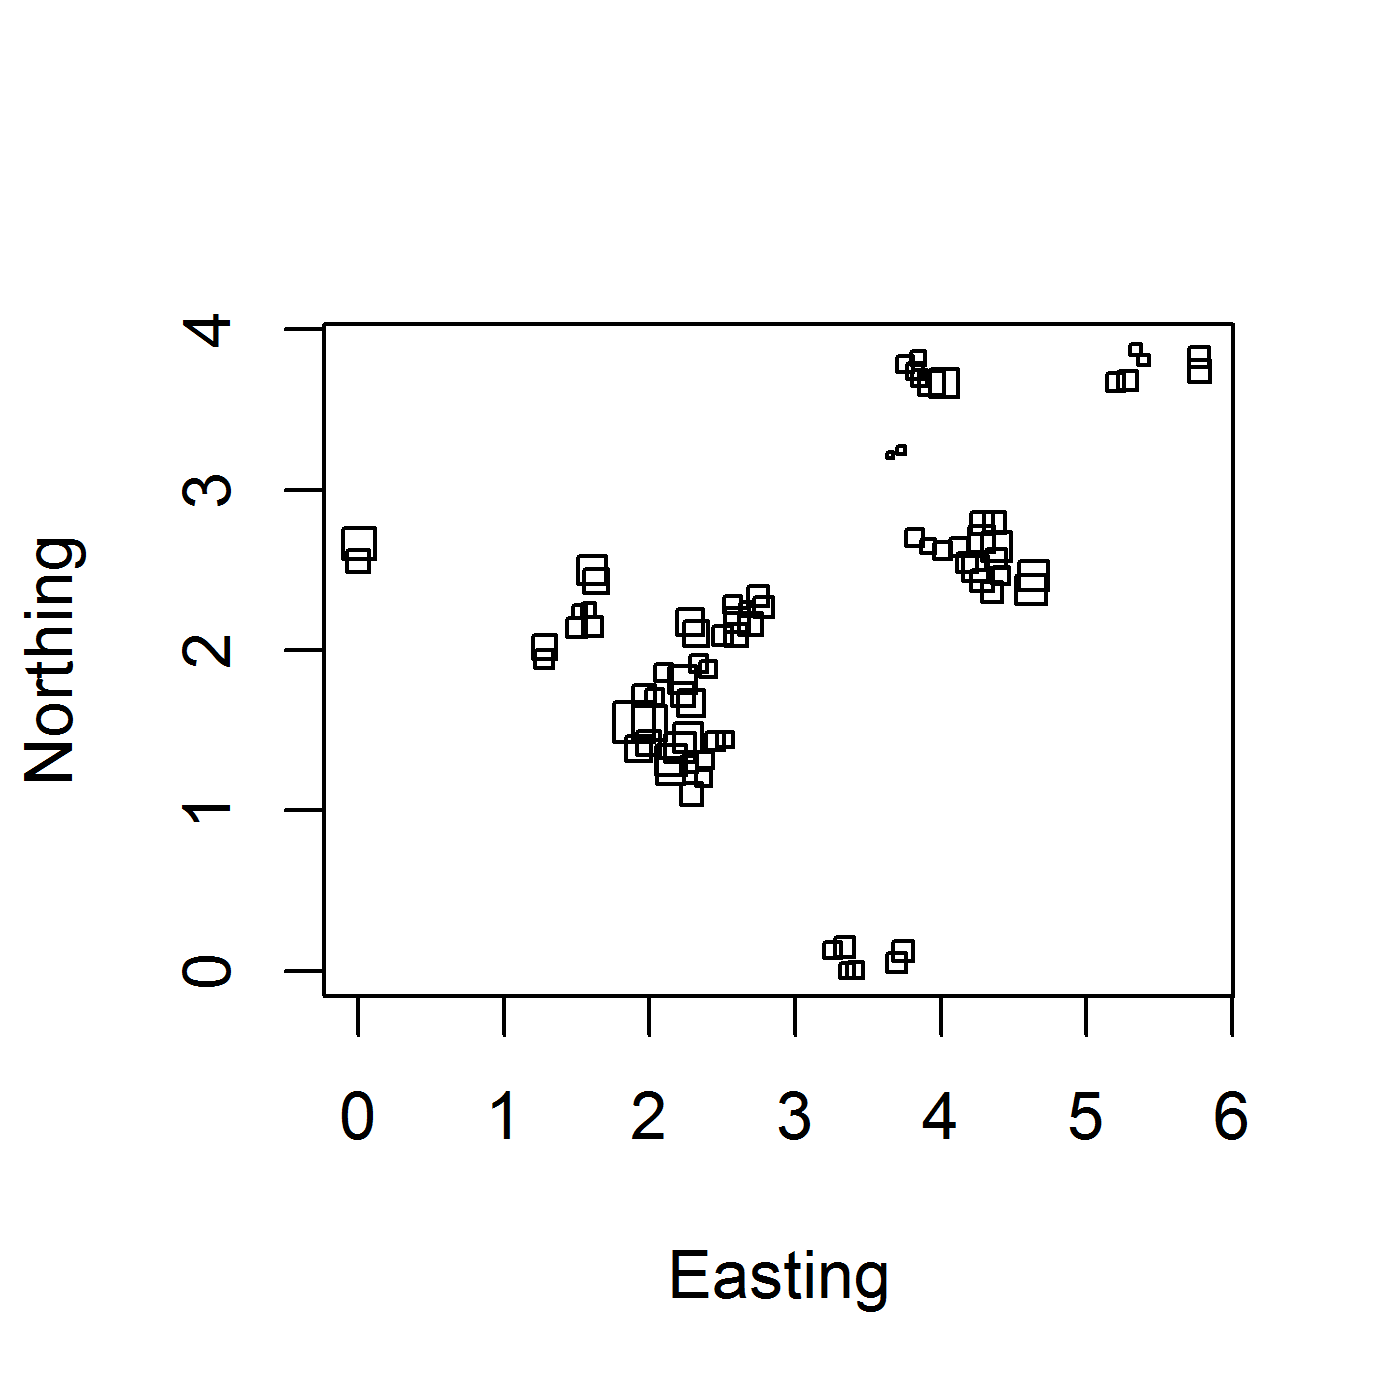
\includegraphics[width=3.5in,height=3.5in]{Ch5/figs/Cap-fragments.png}
\label{poisson-mn.fig.capfrags}
\caption{Relative size and position of 78 forest fragments sampled for
  capricaillie crap.}
\end{figure}


Each of the 44 units
could be sampled by one person in
one day's work (6-8 hours). Within each unit, we focused our search
for droppings on the areas below roosting trees and feeding trees,
respectively, in hiding sites, along internal forest edges, around
root plates and on tree stumps (cf. Jacob et al. 2010). These habitat
elements are the ones preferred by the birds in winter at a small
spatial scale (Bollmann et al. 2005; Mollet unpublished data).
Five spatial units ($I_a$, $S_a$, $S_b$, $H_a$, $T_a$, Table 2) could
not be sampled because of time constraints (too few days with
favorable weather conditions), resulting in 39 units sampled. For the
same reason, three units $(I_b, W_1, W_a)$ were sampled only
once. Access to the area B (Fig. 2) is possible only in late
spring. In 2009, sampling started on 20 April, and the three units in
area B could be sampled only once (rapid snow melting towards the end
of April precluded repetition of sampling here). All other units were
sampled twice.




\subsection{model}

activity centers were uniformly distributed to each of the 78
fragments in proportion to area of the forest patch within which each
fragment was located.


We parameterized activity centers by a discrete state-space with elements
corresponding to the 8 larger fragments. Moreover, home ranges were allocated
to each fragment in  proportion to area. i.e., we assume
define $\lambda_{frag} = A_{frag} \lambda_{0}$, and then:
\[
 N_{frag} \sim Poisson( A_{frag} \lambda_{0} )
\]
This assumption implies the following prior distribution on ${\bf s}_{i}$ (Chapt.
XYZ; Converse and Royle 2012):
\[
{\bf s}_{i} \sim  \mbox{Categorical}(  \pi_{frag} )
\]
with
\[
 \pi_{frag} = \frac{ \lambda_{frag} }{\sum_{frag} \lambda_{frag}}
\]


Observation model:

Each of the 78 fragments is its own sample unit which we index to the
center point of the fragment. No finer scale information is made about
the observation locations.
Let $y_{ij}$ be  the number of times individual $i$ encountered in stand $j$.
Note these are not unique droppings but rather unique clusters of
droppings because a grouse roosting in a tree might leave a number of
droppings and only one of them was sampled\footnote{perhaps this is
  too optimistic of an assessment?}.

\end{comment}



\section{Design 4 -- no location info }

We imagine a series of models for situations where we forget
altogether to record location information within the sample unit. We
further assume the design was such that the sample units represent
contiguous quadrats or at least close enough together so that
individuals may be counted in multiple units. The idea here is that by
being exposed to multiple units, there is a spatial dependence induced
and this spatial dependence provides a little bit more of information
about model parameters. 

We have two specific cases here:
Imagine we have a bunch of quadrats or segments that are contiguous
and we do the surveys like above and record counts PER individual  but
no other sampling information.  Not sure what to do about this.
The other case is that we don't record individual ID at all -- instead
we just have total count frequencies in each plot. 
This model is precisely the one considered by
\citep{chandler_royle:2012} and this is the focus of Chapt. \ref{chapt.nomark}.

Comments on inference for the first situation?




\section{Summary and Outlook}


Searching space for scat is , we imagine, the future of all animal
sampling. 


SCR/DS?